\section{Greedy Problems}

Greedy problems are problems where the optimal solution can always be developed by, at each opportunity, making the choices that provide the most immediate benefit. In other words, the locally optimal choice is also (part of) the globally optimal choice, in all circumstances. Practically, this just means that at any given step of an algorithm, we can reasonably and reliably make the best choice we can.

For example, a simple greedy problem might look like: we are given a binary search tree (remember that elements larger than a given node are always to the right, as a property of binary search trees), and we must print what the maximum element of this tree is.

The greedy solution to this problem is to always traverse to the right of the tree until we end up at a leaf node. This leaf node is the largest element of the tree, guaranteed by the properties of a binary search tree. In greedy terms, starting from the root of the tree, we will greedy move to the largest child node.

While a slightly modified problem stops being greedy: we are given a tree (that isn't necessarily a binary search tree), print what the maximum element of this tree is.
{\centering 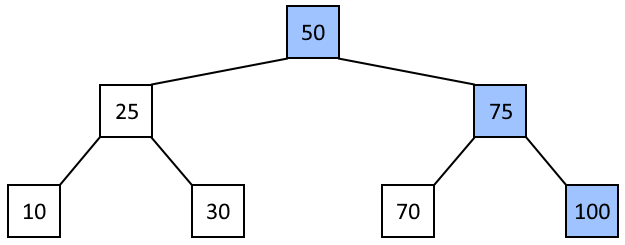
\includegraphics{images/greedy/greedy_tree_1.png}}

Here, this is problem is no longer greedy because we can't reliably say that the largest element is always a child of the larger node. Our greedy solution only worked because we could be guaranteed, at each step, that our locally optimal steps would lead us to the global optimal.
{\centering 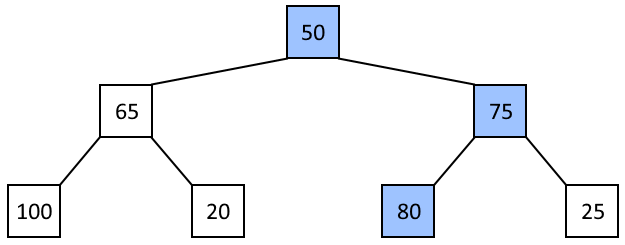
\includegraphics{images/greedy/greedy_tree_2.png}}

\subsection{Knapsack}

\subsection{Coin Change}

\subsection{Interval Cover}